\documentclass{../cheatsheet}
\begin{document}
\setlist[itemize]{left=0pt}
\title{高二 Cheatsheet}
\rowcolors{2}{white}{blue!10}
\renewcommand{\arraystretch}{1.5}
\begin{tabularx}{\columnwidth}{XX}
	\rowcolor{blue!30}
	\multicolumn{2}{l}{\parbox[c][2.5\ht\strutbox][c]{0.9\columnwidth}{\Large 静电场（防止大家忘记）}} \\
    场强定义&$E=\frac Fq$\\
    电势定义&$\varphi = \frac Wq$\\
    电势差定义&$U_{AB}=\varphi_A-\varphi_B$\\
    电场力做功&$W=qU_{AB}=W_A-W_B=\varSigma qE\Delta d$\\
    \multicolumn{2}{l}{\textbf{匀强电场规律}}\\
    电势差与场强关系&$U=Ed$\\
	\multicolumn{2}{l}{\textbf{点电荷}}\\
    库仑定律&$F=\frac{kQq}{r^2}$\\
    点电荷电场强度&$E=\frac{kQ}{r^2}$\\
    点电荷电势&$\varphi=\frac{kQ}{r}$\\
\end{tabularx}
\notice{
    \begin{itemize}
        \item 电势能增加，一般情况下，机械能减少
        \item 判断电势能的增减，可以通过电场力做功，电场力做正功，电势能减小。
        \item 可以通过沿电场线方向电势降低，通过电荷正负与电势的计算式。
        \item 电场力做功注意需要进行投影，也就是$W=qEd\cos\theta$
        \item 电场线与等势面垂直
        \item 在匀强电场中，两点所在直线的场强均匀，可以通过$E^{'}=\frac Ud$求出。
    \end{itemize}
}
\begin{center}
    \includegraphics{}
\end{center}
\begin{tabularx}{\columnwidth}{XX}
	\rowcolor{blue!30}
	\multicolumn{2}{l}{\parbox[c][2.5\ht\strutbox][c]{0.9\columnwidth}{\Large 电路基本元件}} \\
    电流定义式&$I=\frac Qt$\\
    电流决定式&$I = nqSv$\\
    电阻定义式&$R=\frac UI$\\
    电阻决定式&$R=\rho\frac lS$\\
    电容定义式&$C=\frac QU$\\
    电容决定式&$C=\frac{\epsilon S}{4\pi kd}$\\
    电源电动势&$E=\frac{W_{\text{非静电力}}}{q}$\\
\end{tabularx}
\begin{tabularx}{\columnwidth}{XX}
	\rowcolor{blue!30}
	\multicolumn{2}{l}{\parbox[c][2.5\ht\strutbox][c]{0.9\columnwidth}{\Large 闭合电路欧姆定律}} \\
    不含外电路电压&$E=I(R+r)$\\
    不含内阻和电动势&$U=IR$\\
    不含外电阻&$U=E-Ir$\\
    不含电流&$U=E\frac{R}{R+r}$\\
    串联规律&$R=R_1+R_2+\cdots R_n$\\
    并联规律&$\frac1R=\frac1{R_1}+\frac1R_2+\cdots \frac1R_n$\\
\end{tabularx}
\notice{
    \begin{itemize}
        \item 恒压源的正极电势恒定比负极大$E$。
        \item 恒流源干路电流恒定为$I$。（实际上两种电源就是按照上面的原则列欧姆定律方程）
        \item 沿电流方向电势降低
        \item 电势降低量$U=RI$
        \item 对电路中任意节点：$\Sigma I_{in}=\Sigma I_{out}$（如果定义的电流没有流出或者没有流入，那么认为是0。）
        \item 导线的内阻为0，所以导线可以任意长度变化，注意测电阻率时，电阻丝不认为是导线，而是纯电阻。
        \item 理想电流表视为导线，理想电压表视为断路。
        \item 电容器充满电或者稳定状态都视为断路，
        \item 电容器充电过程视为电阻，
        \item 电容器放电视为理想电源。
        \item 断路应该被视为是一个无穷大的电阻接在断路的导线两端。
        \item 任何部分电阻增大都会导致总电阻增大，反之亦然。（该方法可以快速判断总电阻）
    \end{itemize}
}
\begin{tabularx}{\columnwidth}{XX}
	\rowcolor{blue!30}
	\multicolumn{2}{l}{\parbox[c][2.5\ht\strutbox][c]{0.9\columnwidth}{\Large 电表改装}} \\
    电流表简易改装&$R=\frac{I_gR_g}{I_{\text{量程}}-I_g}\approx \frac{I_gR_g}{I_{\text{量程}}}$\\
    电压表简易改装&$R=\frac{U_{\text{量程}}}{I_g}-R_g$\\
    欧姆表改装&$E=i(r+R_g+R_{\Omega}+R_x)$\\
    欧姆表量程刻度&$R_x=\frac{E}{i}-\frac{E}{I_g}=E\frac{I_g-i}{iIg}$\\
    &$R_x=R_{\text{内}}(\frac{I_g}{i}-1)$\\
    欧姆表中值电阻&$R_{\text{中值电阻}}=\frac{E}{I_g}=R_{\text{内}}$\\
\end{tabularx}
\hint{
    多用电表使用，首先进行机械调零，旋转机械调零螺丝让指针指到电流表的0刻度线。注意这个名字，机械调零螺丝，欧姆调零旋钮。\\
    如果使用欧姆表测电阻，\\
    1. 首先选择合适挡位\\
    2. 进行欧姆调零，红黑表笔短接，\\
    3. 旋转欧姆调零旋钮让指针指到电流表满偏位置（同时也是欧姆表0刻度线）。\\
    每次换挡都需要进行欧姆调零。

}
\hint{
    上面的改装原理可以解释为什么电流表和电压表表盘是均匀的，而欧姆表的表盘不均匀。\\
    通过电流表改装的公式可以得到：
    \[\frac{i}{I}=\frac{R}{R+R_g}\]
    \[\frac{i_{\text{表头电流}}}{I_{\text{干路电流}}}=\frac{I_g}{I_{\text{满偏}}}\]
    即，改装后的电流表，表头电流与干路电流成正比，那么可以利用表头读数计算干路电流，并且是线性的关系。\\


    通过电压表改装的公式可以得到：
    \[i=\frac{U_\text{总}}{R+R_g}\]
    即总电压与表头电流成正比，那么可以利用表头读数计算总电压，并且是线性的关系。\\
    
    
    通过欧姆表改装的公式可以得到：
    \[i=\frac{E}{R_{\text{内}}+R_x}\]
    即，表头电流与被测电阻成反比，表盘才会不均匀，并且电阻越大，电流变化幅度越小，左边的刻度偏角间隔就会越小。\\
}
\begin{tabularx}{\columnwidth}{XX}
	\rowcolor{blue!30}
	\multicolumn{2}{l}{\parbox[c][2.5\ht\strutbox][c]{0.9\columnwidth}{\Large 用电器功率和电源功率}} \\
    电功率定义式&$P=UI$\\
    \multicolumn{2}{l}{\textbf{用电器功率}}\\
    纯电阻功率&$P=P_{\text{热}}=I^2R=\frac{U^2}{R}$\\
    非纯电阻总功率&$P=UI$\\
    非纯电阻热功率&$P=I^2R$\\
    非纯电阻输出功率&$P=UI-I^2R$\\
    \multicolumn{2}{l}{\textbf{电源功率}}\\
    电源总功率&$P=EI=\frac{E^2}{R+r}\le \frac{E^2}{r}$\\
    电源热功率&$P=I^2r=(\frac{E}{R+r})^2r\le \frac{E^2}{r}$\\
    电源输出功率&$P=UI=(E-Ir)I=(\frac{E}{r}-I)Ir$\\
    包含纯电阻电源输出功率&$P=(\frac{E}{R+r})^2R=\frac{E^2}{R+\frac{r^2}{R}+2r}\le \frac{E^2}{4r}$\\
\end{tabularx}
\hint{
    \begin{itemize}
        \item 正常工作意味着用电器的全部物理量为额定值
        \item 电动机这样的非纯电阻元器件，不能正常工作，可以看作纯电阻。
        \item 灯泡虽然会发热，但是仍然看成定值电阻。
        \item \textbf{不要使用非纯电阻两端电压得到电流或者电阻。$r\neq \frac UI$}
        \item 非纯电阻的内阻也不要与其他电路电阻进行串并联。
    \end{itemize}
}
{
    \centering
    \textbf{电源总功率与电流图像}\\
    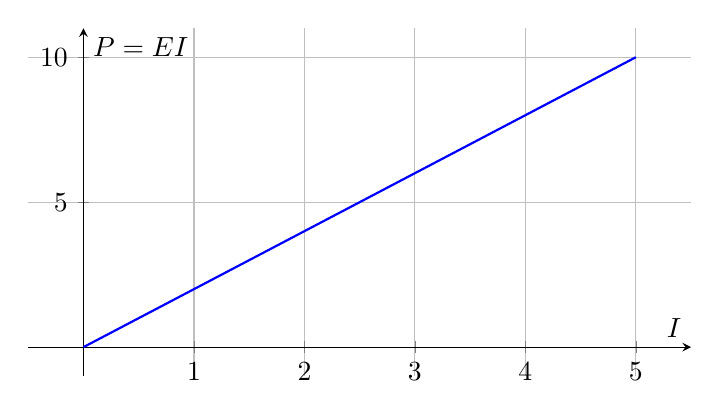
\begin{tikzpicture}
        \begin{axis}[
            width=10cm, height=6cm,
            axis lines=middle,
            xlabel={$I$},
            ylabel={$P = EI$},
            xmin=0, xmax=5,
            ymin=0, ymax=10,
            grid=both,
            samples=100,
            domain=0:5,
            enlargelimits
        ]
        \addplot[blue, thick] {2*x}; % E = 4V 为示例
        \end{axis}
    \end{tikzpicture}\\
    \textbf{电源总功率与外电阻图像}\\
    \begin{tikzpicture}
        \begin{axis}[
            width=10cm, height=6cm,
            axis lines=middle,
            xlabel={$R$},
            ylabel={$P = \dfrac{E^2}{R + r}$},
            xmin=0, xmax=6,
            ymin=0, ymax=5,
            grid=both,
            samples=200,
            domain=0:6,
            enlargelimits,
            legend pos=south east
        ]
        \addplot[red, thick, domain=0:10] {4/(x + 1)}; % E = 4, r = 4 为例
        \end{axis}
    \end{tikzpicture}\\
    \textbf{电源热功率与电流图像}\\
    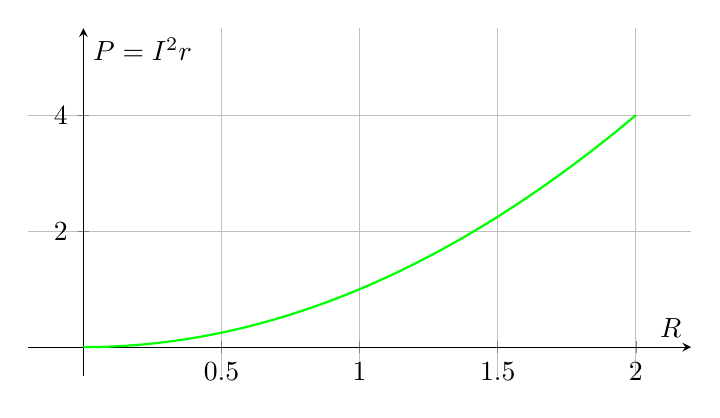
\begin{tikzpicture}
        \begin{axis}[
            width=10cm, height=6cm,
            axis lines=middle,
            xlabel={$R$},
            ylabel={$P = I^2r$},
            xmin=0, xmax=2,
            ymin=0, ymax=5,
            grid=both,
            samples=200,
            domain=0:2,
            enlargelimits,
            legend pos=south east
        ]
        \addplot[green, thick, domain=0:2] {(x*x)*1)}; % E = 4, r = 4 为例
        \end{axis}
    \end{tikzpicture}\\
    \columnbreak
    \textbf{电源热功率与外电阻图像}\\
    \begin{tikzpicture}
        \begin{axis}[
            width=10cm, height=6cm,
            axis lines=middle,
            xlabel={$R$},
            ylabel={$P = \dfrac{E^2}{(R + r)^2}r$},
            xmin=0, xmax=2,
            ymin=0, ymax=5,
            grid=both,
            samples=200,
            domain=0:6,
            enlargelimits,
            legend pos=south east
        ]
        \addplot[black, thick, domain=0:2] {(4/(x + 1)^2};
        \end{axis}
    \end{tikzpicture}\\
    \textbf{电源输出功率与电流图像}\\
    \begin{tikzpicture}
        \begin{axis}[
            width=10cm, height=6cm,
            axis lines=middle,
            xlabel={$R$},
            ylabel={$P = (\dfrac{E}{r}-I)Ir$},
            xmin=0, xmax=2,
            ymin=0, ymax=1,
            grid=both,
            samples=200,
            domain=0:2,
            enlargelimits,
            legend pos=south east
        ]
        \addplot[blue, thick, domain=0:2] {x*(2-x)}; 
        \end{axis}
    \end{tikzpicture}\\
    \textbf{电源输出功率与外电阻图像}\\
    \begin{tikzpicture}
        \begin{axis}[
            width=10cm, height=6cm,
            axis lines=middle,
            xlabel={$R$},
            ylabel={$P = \dfrac{E^2}{(R + r)^2}R$},
            xmin=0, xmax=6,
            ymin=0, ymax=1,
            grid=both,
            samples=200,
            domain=0:6,
            enlargelimits,
            legend pos=south east
        ]
        \addplot[red, thick, domain=0:6] {4/(x+1/x+2)};
        \end{axis}
    \end{tikzpicture}\\
}
\begin{tabularx}{\columnwidth}{XX}
	\rowcolor{blue!30}
	\multicolumn{2}{l}{\parbox[c][2.5\ht\strutbox][c]{0.9\columnwidth}{\Large 电路实验}} \\
    电流表外接&$R_x<\sqrt{R_VR_A}$\\
    通过试触法判断&$\frac{\Delta I}{I} < \frac{\Delta U}{U}$\\
    电流表内接&$R_x>\sqrt{R_VR_A}$\\
    通过试触法判断&$\frac{\Delta I}{I} > \frac{\Delta U}{U}$\\
    滑动变阻器限流解法&$R_{\text{滑动变阻器}}$略大于或者为3-5倍 $R_x$\\
    滑动变阻器分压解法&$R_{\text{滑动变阻器}}<R_x$\\
    &U需要从0开始\\
\end{tabularx}
\notice{
    \begin{itemize}
        \item 电表量程选择时，可以略超量程，但是不能选择过大的量程
        \item 连接电路的导线时请按照电路图进行。
    \end{itemize}
}
\end{document}
